\documentclass{sigchi}

%Conference
\conferenceinfo{Ortega '19,}{December  18, 2019, Fort Collins, CO, USA}

% page numbers for the camera ready copy
\pagenumbering{arabic}

% Load basic packages
\usepackage{balance}       % to better equalize the last page
\usepackage{graphicx}      % for EPS, load graphicx instead 
\usepackage[T1]{fontenc}   % for umlauts and other diaeresis
\usepackage{txfonts}
\usepackage{mathptmx}
\usepackage[pdflang={en-US},pdftex]{hyperref}
\usepackage{color}
\usepackage{booktabs}
\usepackage{textcomp}
\usepackage{subfig}
\usepackage{microtype}        % Improved Tracking and Kerning
\usepackage{ccicons}          % Cite your images correctly!

\def\plaintitle{A Methodology for the Simultaneous Monitoring of Bridge Load and Induced 3-D Displacement using Unmanned Aerial Vehicles (UAVs) with Real-Time Data Interpretation User Study}
\def\plainauthor{Brandon J. Perry}
\def\emptyauthor{}
\def\plainkeywords{Real-Time Data Interpretation; Structural Health Monitoring; 3-D Bridge Displacement; UAV Bridge Inspection.}
\def\plaingeneralterms{Documentation, Standardization}

% Define a global style for URLs, rather that the default one
\makeatletter
\def\url@leostyle{%
  \@ifundefined{selectfont}{
    \def\UrlFont{\sf}
  }{
    \def\UrlFont{\small\bf\ttfamily}
  }}
\makeatother
\urlstyle{leo}

% To make various LaTeX processors do the right thing with page size.
\def\pprw{8.5in}
\def\pprh{11in}
\special{papersize=\pprw,\pprh}
\setlength{\paperwidth}{\pprw}
\setlength{\paperheight}{\pprh}
\setlength{\pdfpagewidth}{\pprw}
\setlength{\pdfpageheight}{\pprh}

\definecolor{linkColor}{RGB}{6,125,233}
\hypersetup{%
  pdftitle={\plaintitle},
  pdfauthor={\plainauthor},
  pdfkeywords={\plainkeywords},
  pdfdisplaydoctitle=true, 
  bookmarksnumbered,
  pdfstartview={FitH},
  colorlinks,
  citecolor=black,
  filecolor=black,
  linkcolor=black,
  urlcolor=linkColor,
  breaklinks=true,
  hypertexnames=false
}

% End of preamble. Here it comes the document.
\begin{document}

\title{\plaintitle}
\numberofauthors{1}
\author{
  \alignauthor{Brandon J. Perry\\
    \affaddr{Colorado State University}\\
    \affaddr{Fort Collins, Colorado, USA}\\
    \email{bjperry@colostate.edu}}\\}

\maketitle

\begin{abstract}
    UPDATED---\today. Fully understanding bridge performance during traffic is critical for effective condition assessment. Modern structural health monitoring (SHM) has enabled measurements of traffic loads and dynamic responses; however, challenges still exist for accurately synchronizing the two inputs. Recently, with advancements in unmanned aerial vehicles (UAVs) technology, UAVs can hover at specified heights and key locations to provide high-quality sensory data. By leveraging UAVs and image computation, this study proposes a UAV-based SHM framework to track vehicular loading and measure the 3-D displacement of a bridge simultaneously. In the proposed methodology, multiple UAVs will hover adjacent to a bridge to collect data of the moving traffic and structural response. Through a case study, the potential of synchronizing dynamic traffic loads and 3-D structural response is demonstrated. Lastly, a user study is presented to determine the importance of real-time information compared to post-process information for civil engineers in the field. 
\end{abstract}

% ACM Classfication

\begin{CCSXML}
<ccs2012>
<concept>
<concept_id>10003120.10003121</concept_id>
<concept_desc>Human-centered computing~Human computer interaction (HCI)</concept_desc>
<concept_significance>500</concept_significance>
</concept>
<concept>
<concept_id>10003120.10003121.10003125.10011752</concept_id>
<concept_desc>Human-centered computing~Haptic devices</concept_desc>
<concept_significance>300</concept_significance>
</concept>
<concept>
<concept_id>10003120.10003121.10003122.10003334</concept_id>
<concept_desc>Human-centered computing~User studies</concept_desc>
<concept_significance>100</concept_significance>
</concept>
</ccs2012>
<ccs2012>
<concept>
<concept_id>10010405.10010432.10010439</concept_id>
<concept_desc>Applied computing~Engineering</concept_desc>
<concept_significance>500</concept_significance>
</concept>
</ccs2012>
\end{CCSXML}

\ccsdesc[500]{Applied computing~Engineering}
\ccsdesc[100]{Human-centered computing~User studies}
\ccsdesc[100]{Human-centered computing~Human computer interaction (HCI)}

% Author Keywords
\keywords{\plainkeywords}

% Print the classification codes
\printccsdesc

\section{Introduction}

Understanding the dynamics of bridges is critical for evaluating long-term structural performance and decision-making regarding the operation of the structure. However, there still exist two challenges when studying the dynamics of bridges. Firstly, the constantly changing and fluctuating dynamic loads on the structure are difficult to measure and thus are often treated as unknowns. Secondly, the measurement of dynamic displacement is more difficult compared to the acceleration. The total displacements cannot be fully recovered from accelerometers of inertial measurement units due to the inability to solve for the constants of integration when double integrating the accelerations. Overcoming these two challenges would help engineers, researchers, and city planners to better understand the performance of the structure and make the most informed decisions about maintenance and operations.

Traditionally, accelerometers have been deployed to measure the dynamic response of bridges. However, these systems require a large number of sensors, careful pre-planning of the sensor placement, and management of the wires if a wired system or synchronization of the sensors if a wireless system is adopted. For instance, Linderman et al. attached twenty-six accelerometers on the structure to measure the necessary dynamic response of I-35W Saint Anthony Falls Bridge in Minneapolis, Minnesota \cite{Linderman2019DisplacementSystem}. Although the accelerometer sensors provided a wealth of information that is not typically available for large-scale bridges, the scale of the sensory array may impose logistical problems for the bridge owners and researchers. Several of the sensors lost communication due to a number of reasons. Moreover, once the sensors were attached, they were not easily able to be relocated if a different, critical location was found. Furthermore, the entire undertaking did not measure the induced dynamic loads of the structure.

Recently, Unmanned Aerial Vehicles (UAVs) are being deployed to assist bridge inspectors and managers. UAVs have the potential to provide information from various difficult-to-access locations of a bridge on a faster, more cost-effective, and safer platform when compared to traditional techniques. Some studies have already explored the possibility of utilizing UAVs as ``eyes-in-the-sky'' to assist inspectors in the field \cite{Gillins2016,Wells2018}. These studies investigate the viability of using UAVs equipped with optical sensors to assist inspectors and show the possibility for future implementation for bridge inspection. As the size and capabilities of various sensors improve, a more diverse application of UAV sensors become possible. This study proposes equipping a UAV with various optical and infrared sensors to capture both the dynamic loading and structural response of bridges. Currently, there are few sensors that can potentially be used to collect this information in a robust manner. This paper examines the use of an Intel$^{\text{\textregistered}}$ RealSense D35 depth sensor in conjunction with typical optical cameras attached to a UAV. The RealSense sensor was initially developed for human-computer interactions in 3-D environments. Applying this sensor to civil infrastructure, it can tackle the measurements of the displacement of a bridge. To provide the live load information, a truck-tracking procedure based on computer vision is developed which allows a UAV to follow a truck from a weigh station to the bridge location.

There is some research on using UAVs to track the displacements of a bridge. These UAVs systems rely on an optical sensor on a UAV and a painted speckle pattern on a bridge to measure dynamic displacement \cite{Kalaitzakis2019,Catt2019Development}. Baqersad et al. mounted two cameras with known distances apart and known camera parameters to measure the deformations of a deformable board. The proposed algorithm processes the speckled pattern placed on the board to accurately measure the precise 2-D deformation and movement of the speckles. Moreover, \cite{Kalaitzakis2019} implemented a similar set up to measure strains of a concrete beam during a four-point loading test. Lastly, Instron Testing Equipment has a commercial software to measure strains during tensile tests using similar techniques of measuring the displacements of a speckle pattern on a specimen \cite{Instron2017}. However, these three systems require an applied speckle pattern to be manually drawn on the specimen prior to the tests. Implementing this type of system in the real-world might be difficult due to the large-scale of the structures and the workforce required. Additionally, the systems measure only the 2-D planar deformation of the object; the plane that is perpendicular to the camera. It is not able to measure the full, 3-D movement of an object. Recently, several products have made an appearance on the market place which can measure displacements using a virtual speckle pattern instead of the real speckle patterns used in the previous studies. However, these systems have a limitation of only being able to measure 1-D, i.e., the distance from the sensor to the object (depth). Considering the advantages and shortcomings of the aforementioned techniques, this study proposes to integrate the 2-D planar measurement and 1-D depth measurement to measure all 3-D dynamic displacements.

Intel's RealSense senor and Microsoft's Kinects sensor implement a virtual speckle pattern onto an object to measure the depth from the camera to an object. It incorporates two infrared cameras and an infrared laser projector. The laser projects the speckle pattern on a subject. Next, the two infrared cameras on each side of the laser projector capture the reflection of the speckle pattern. The two infrared cameras are rigidly attached to the laser source, and, with the camera matrix known, are able to track each speckle and calculate the depth of the object from the sensor. 

Utilizing the virtual speckle pattern technique built into the Intel's or Microsoft's sensors systems have been successfully applied in human-computer interactions and medical fields. Nguyen et al. used two Microsoft's Kinects sensors and the virtual speckle pattern to measure the displacements in a variety of objects and was able to measure the breath rate of a chest and the pulse from a subject's neck with a high accuracy \cite{Nguyen2018}. Aoki et al. created a virtual grid using a green laser to project a pattern on a subject's chest to measure with high accuracy the heartbeat of a subject \cite{Aoki2018StudySensor}. Within these two studies, the placement and movement of the sensors were highly controlled and measured. If these systems were implemented on a UAV where there is random vibration and/or movement due to the instability of the UAV hovering, there could be significant error induced in the measurements. Therefore, there needs to be a system developed that can either overcome or compensate the vibrations and/or movements of the projector or sensors during the tests. 

This paper presents a proof-of-concept study of a framework to 1) measure the 3-D displacement of a structure using an optical sensor for 2-D planar movement and an Intel$^{\text{\textregistered}}$ RealSense D35 Sensor for 1-D depth movement, 2) tracks the imposed loading with a truck-tracking procedure with UAVs, as well as, 3) perform a user study of the effectiveness of providing real-time data to civil engineers in the field. The paper will be organized to first examine the overall framework and real-world implementation. Next, three sections are presented to introduce the algorithms of the truck-tracking, 2-D planar movement, and 1-D depth movement of an object and demonstrate the implementation of the proposed three algorithms, respectively. Lastly, a user-study will be presented to understand whether the difficulties of providing real-time data to engineers in the field is worth the added expense and complication as opposed to post-processed data interpreted interpreted in office or in the field. The full user-study will be presented in the last section.

\section{Overview of Proposed Framework and Its Real-World Implementation}

The three modules of the framework will be presented through a proof-of-concept study. The first module is ``truck-tracking'' which follows a truck to measure the dynamic loading. The second module is tracking the 2-D planar movements of an object using a typical RGB/optical sensor on a UAV. The third module is to measure the 1-D depth movement of an object using the RealSense sensor. The accuracy of the implementation of the three modules will be examined.

First, to measure the dynamic loading of the structure in order to build an input-output model, it is proposed to implement a ``truck-tracking'' system. A UAV is synced to the weigh-in-motion sensors currently installed in the United State's interstate infrastructure. Originally developed and used to ensure compliance with state and federal regulations, the information can be collected and used in the framework. The weight of a large truck provides the critical live loads of a structure, which is often the most relevant load regarding the operation of the infrastructure. Once the weight is collected, a UAV tracking system is used to follow the weighed truck from the weighing area to the bridge and follow the truck as it passes over the bridge.

Next, the feasibility of measuring the 3-D dynamic response of a bridge will be presented. The 3-D measurement is accomplished by two modules. The first module uses RGB/optical sensors on a UAV to track and measure 2-D planar dynamic displacement perpendicular to the camera. The second module uses the RealSense sensor to measure depth from the sensor to a region of interest. A UAV equipped with a set of RealSense sensors will hover adjacent to a bridge to measure the displacement of the structure through tracking the movement of projected the virtual speckle pattern. Integrating the 2-D planar motion with the 1-D depth motion information, the total 3-D dynamic displacement of the bridge is known. These three modules together will enable simultaneous measurement of both dynamic loading and displacement on a bridge, which will allow in-depth analysis of the structural dynamic performance and enhance the accuracy of the condition evaluation of bridges. The three proposed modules will be discussed in the following sections in detail with results from case studies presented.

Lastly, providing real-time information to engineers in the field creates complications with data transmission and synchronization. These problems associated with providing real-time information is attainable; however, comes at an expense for added equipment and complication of the framework. Therefore, a user study is presented to understand whether an engineer can effectively interpret real-time information with visual and auditory distractions of moving vehicles.

\section{Truck-tracking Module}

To provide the live loading of a bridge in order to allow for a full input-output analysis, a truck is tracked from the weigh-in-motion station until it passes over the bridge. For this implementation, it is assumed that the weigh-in-motion stations are in close proximity to a bridge of interest. However, as a bridge becomes more remote, the live load truck tracking may not be possible due to the energy required to track a truck over a longer distance. Tracking of objects is currently a trivial task in computer vision. In this implementation, a ``Minimum Output Sum of Squared Error'' (MOSSE) filter is used. The MOSSE filter is created by a pixel-wise division of an image with only a Gauss point placed at the known location of the object and the entire frame from a video in the frequency domain \cite{Bolme2010VisualFilters}. Once the filter is obtained, it is multiplied by the next frame to produce a new Gauss point of where the object is. The filter is then updated and the process is continued. It requires only the initial position of the object being tracked and requires the object to move continuously from frame to frame. It has proved to be a highly effective, fast, and accurate technique to track an object in a video and can be implemented in real-time. Connecting with a weigh-in-motion system, the weight of a truck is associated with the position of the vehicle through the tracking algorithm. The truck's load will be known as it crosses over the structure. 

To track and follow a truck, the algorithm and technique are fairly robust and well studied. The technique was demonstrated with a UAV flying about 90-\textit{meters} above ground level and followed a truck on a road.

\begin{figure}[ht]
    \centering
    \includegraphics[width=0.9\columnwidth]{Figures/truck_tracking.png}
    \caption{UAV Tracking a truck at  90-\textit{meters} Above Ground Level}~\label{fig:truck}
\end{figure}

\section{2-D Planar displacement measurement Module}

With the truck-tracking algorithm implemented to measure the dynamic traffic load, the UAV sensors can be used to measure the displacement of the bridge simultaneously. Two techniques are integrated to find the dynamic 3-D displacement of a bridge. The first algorithm is an implementation of a 2-D measurement technique onto an optical sensor attached to a UAV \cite{Kalaitzakis2019,Catt2019Development}. Measuring the 2-D planar motion perpendicular to the sensor requires tracking of key-points within an image over time to calculate the movement. This type of technique has shown potential using stationary cameras and sensors; however, when applying these techniques to the camera attached to UAVs, a problem arises. There are movement and instability with the UAV as it hovers. Although the UAV may remain stable in the air, there is slight drifting and movement of the sensor and error is imposed. A correction of this error must be applied to get the movement of the actual object. In the following, the algorithm to track 2-D planar motion and the treatment of correcting the error due to the UAV movement are introduced.

The proposed 2-D displacement tracking technique uses the scale-invariant feature transform (SIFT) algorithm to identify key-points and their associated descriptors within a region of interest (ROI)\cite{Lowe1999}. SIFT key-points are irrelevant of scale and orientation and prove to work well in a variety of applications. SIFT key-points track the subpixel locations of key-points within an image. The number of SIFT key-points within an ROI depends on the size, resolution, and texture of the object. Smoother objects such as concrete tend to not reveal many key-points in an image, thus may introduce difficulties for the following motion tracking. Therefore, to overcome this problem, an artificial pattern (i.e. the speckle pattern) is implemented to provide areas of interest for the SIFT algorithm to identify more key-points. Performing this SIFT analysis on a frame-by-frame basis of video collected by a UAV allows tracking on a subpixel level of the area of interests. Next, using a brute force technique, the key-points and its related descriptors are matched with an initial frame for a point of reference. The matches are then sorted and the top five matches are used for the analysis. Since the selected ROI is relatively small, averaging the top five matches provide a measurement of the location of the ROI. Comparing this average with the initial frame identifies the movement of the ROI from frame to frame. At first appearance, it may seem best to match the same identified key-points from frame to frame; however, during the implementation, it was found that averaging produced more precise results. This is probably due to the variation in the accuracy of the matches. For instance, for different frames, different key-points may be better and more precisely matched, and, therefore, the related movement is better estimated by taking the average.

As discussed earlier, the movement of the UAV during flight introduces error on the 2-D motion measurement results. Therefore, it is necessary to correct or compensate for the UAV's movement. To overcome the movement of the UAV during flight, SIFT key-points of the background are also found and tracked from frame to frame. Assuming the movement of the background is due only to the movement of the UAV, the background movement is subtracted out from the movement of the object and the true movement of the object is found. 

\subsection{Case Study}

To test this algorithm, the dynamic displacement measurement of a transmission line was studied. Although the methodology was originally developed for bridge application, the transmission line test was used as a proof of concept because of the available experimental opportunity. Another research group from Colorado State University was conducting tests on the vibration of a transmission line under blast-induced excitation to study the mechanism of how the transmission line dynamically reacted to the blast. Therefore, it provided a good experimental opportunity for the authors to test the developed UAV-based dynamic displacement measurement algorithm. Since both transmission lines and bridges are line-like structures, the feasibility tested on a transmission line implies the potential of the method for bridge application. The experimental setup is shown in Figure \ref{fig:blast}.

\begin{figure}[ht]
    \centering
    \subfloat[Side View of Set Blast Set-Up]{\includegraphics[width=0.9\linewidth]{Figures/blast.PNG}}
    \\
    \subfloat[View from UAV of Blast Test Set-Up] {\includegraphics[width=0.9\linewidth]{Figures/blast22.png}}
    \caption{Experimental Set-up of Using a UAV to Measure Dynamics of Transmission Line}~\label{fig:blast}
\end{figure}

Since the transmission line was a relatively smooth, and narrow surface, few SIFT key-points were produced within a small ROI. To provide better SIFT points identification, an artificial pattern (i.e. the speckle pattern) was manually imposed on the transmission line. The pattern was a random black and white polka dot pattern which provided high contrast for identification of SIFT key-points. The dot pattern was printed on paper and wrapped around the transmission line. Since the paper was thin, light-weight, and matched the shape of the transmission line, it was assumed that any error imposed by the artificial speckle pattern by stiffening or restricting the movement of the wire was negligible. The UAV was flown about 6-\textit{meters} above the transmission line and about 7.5-\textit{meters} above ground level. Using a DJI Mavic 2 Zoom with the 2X optical zoom provided a ground-sampling distance of 0.13-\textit{cm/pixel}. Next, the same random speckle polka dot pattern was secured to the ground below the transmission line. This was used as a reference to correct the movement of the UAV as previously mentioned.

The movement of the transmission line and the movement of the stationary ROI were measured and subtracted to get the true movement of the transmission line. Since it is not feasible to install accelerometer or GPS sensors on the thin power line to do a comparison study, the ground-truth data is currently not available; however, the measurement results appeared consistent with what was observed, which indicates the initial success of this method. The resulting, estimated dynamic displacement of the transmission line captured by the UAV is shown in Figure \ref{fig:dis-blast}. The power spectral density estimated using a Fast Fourier Transform is also shown, where the dominant frequency is 2.80-\textit{Hz}.

\begin{figure}[ht]
    \centering
    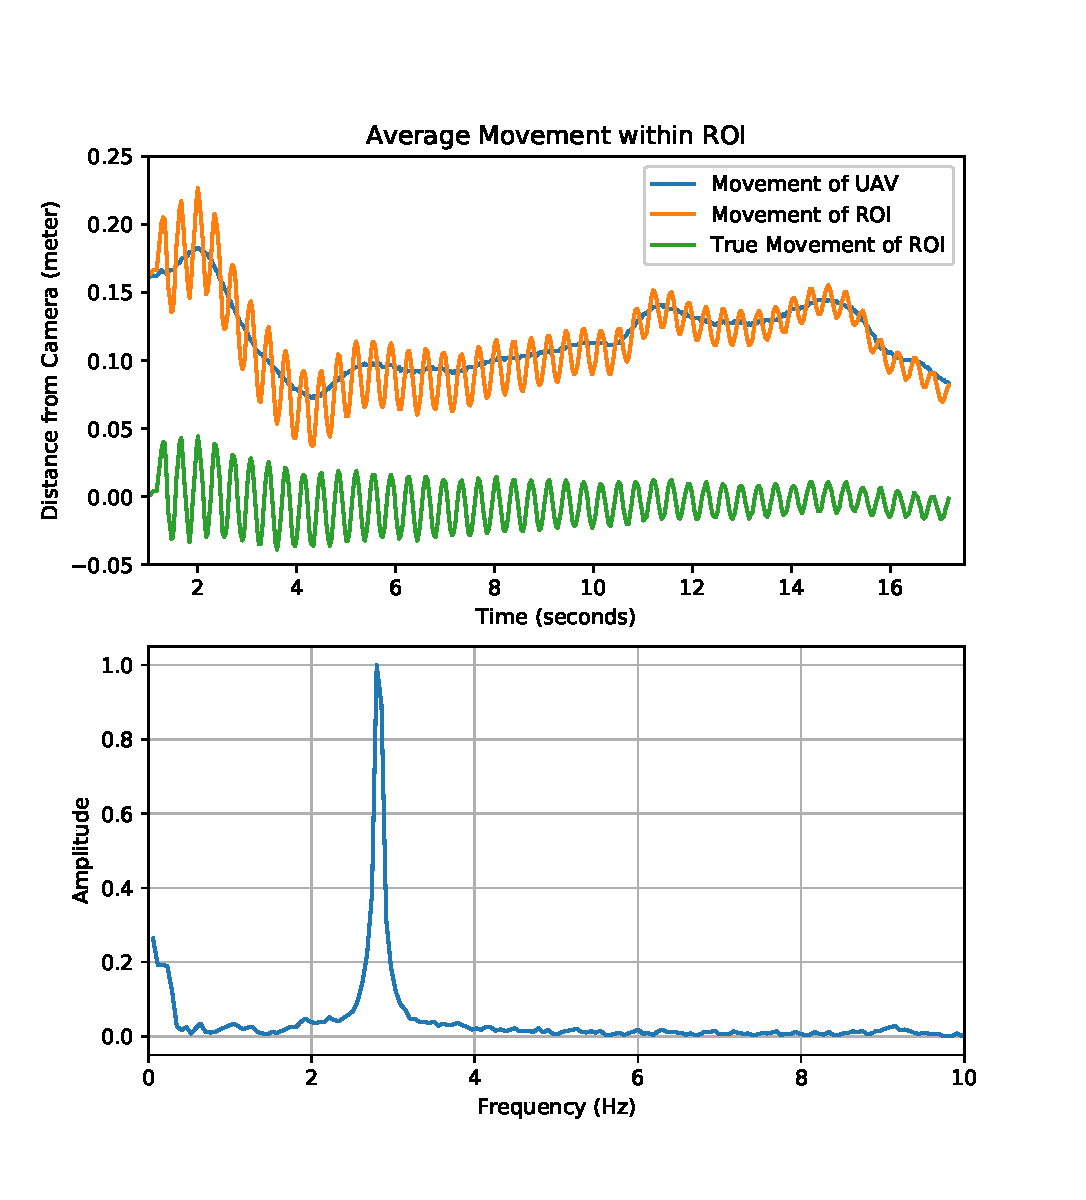
\includegraphics[width=.9\columnwidth]{Figures/blast_graph}
    \caption{2-D Planar Displacement of the Transmission Line recorded by a UAV}~\label{fig:dis-blast}
\end{figure}

\section{1-D Depth Measurement Module}

An Intel RealSense Depth Camera was used. This camera was initially developed to measure and track hand motions to interact with computers within virtual environments with virtual reality head-mounted displays. The camera casts an infrared laser that projects a virtual speckle pattern onto an object. In addition to an RGB camera, two infrared cameras are attached to the sensor which record the reflection of the laser pattern. The camera's ``camera matrix'' which consists of the intrinsic and extrinsic information is known and constant. Knowing the ``camera matrix,'' the speckle pattern of the infrared laser is tracked and measured. Using Intel's RealSense SDK 2.0, an algorithm was developed which measured the distance from an object to the sensor and the power spectral density of the obtained time history of displacements was estimated using a Fast Fourier Transform. After adjusting the camera's parameters, a small ROI is selected which is small enough to be considered as a point on the object. In this way, the dynamic displacement of the object in the depth direction from the sensor to ROI is measured.

\subsection{Case Study}

To test the proposed method, a simple, small scale experiment was set up. Using a custom-built shake-table which will produce known, and controlled displacements, a prismatic, rigid structure was secured onto it. The excitation of the shake table was varied between 0.50 - 2.00-\textit{Hz}. The cameras were set up perpendicular to the rigid structure at a distance approximately 0.5\textit{-meters} away in a defined x- and y-direction. The cameras recorded the two infrared cameras and the depth was calculated. The max frame-rate of the camera is 30\textit{-fps}. According to the classic Nyquist–Shannon sampling theorem, the sampling frequency needs to be at least twice the maximum frequency of the vibration to faithfully record the signal. So the sampling frequency of 30\textit{-fps} is large enough to capture vibrations up to 15\textit{-Hz}. For the tested systems, the maximum frequency of vibration is less than 2\textit{-Hz}; therefore, the camera records at a sufficient rate to provide enough sampling points to measure the frequency of vibration. These measured vibration frequencies from the RealSense sensor were compared to an accelerometer secured onto the shake-table. The results for two tests with different excitation frequencies are shown in Figure \ref{fig:Freq}. The results for all five of the tested frequencies are compared with those obtained from the accelerometer in Table \ref{table:Results}. 

\begin{figure}[ht]
    \centering
    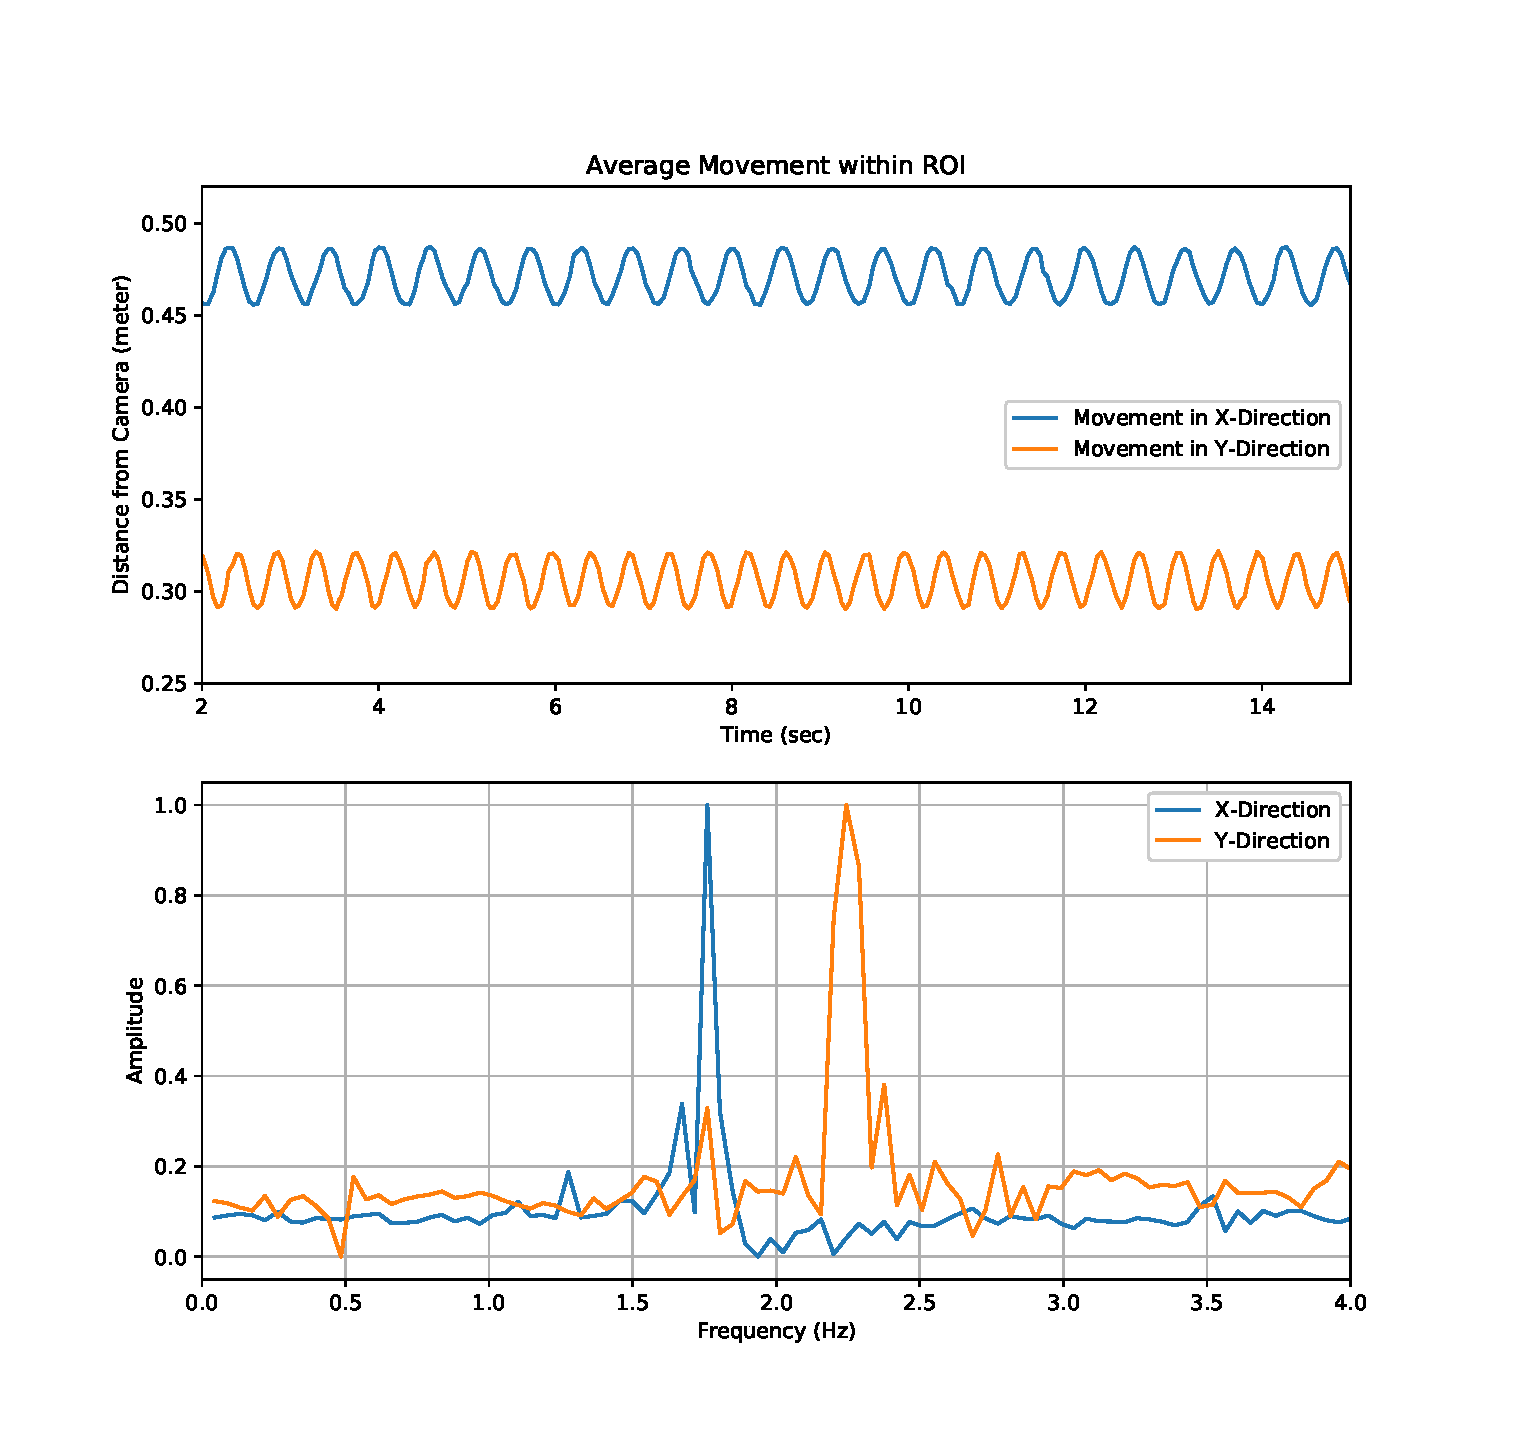
\includegraphics[width=.9\columnwidth]{Figures/6}
    \caption{Displacement Time History and Frequency Component obtained from the RealSense Sensor}~\label{fig:Freq}
\end{figure}

\begin{table}[t]
    \centering
    \begin{tabular}{@{}rccc@{}}
    \toprule
    \multicolumn{1}{l}{} Test & \begin{tabular}[c]{@{}c@{}}Ground Truth\\ Frequency\end{tabular} & \begin{tabular}[c]{@{}c@{}} Frequency from \\ RealSense Sensor\end{tabular} & \begin{tabular}[c]{@{}c@{}}Percent\\ Different\end{tabular} \\ \midrule
    1 & 0.49 & 0.50 & 0.98\% \\
    2 & 1.48 & 1.50 & 1.68\% \\
    3 & 1.99 & 2.00 & 0.55\% \\
    4 & 1.76 & 1.76 & -0.13\% \\
    5 & 2.23 & 2.25 & 1.13\% \\ \bottomrule
    \end{tabular}
    \caption{A Comparison between Displacement and Acceleration Measurements}~\label{table:Results}
\end{table}

From the comparison results listed in Table \ref{table:Results}, the percent difference from the accelerometer and the RealSense camera are less than 2\%. This demonstrates the efficacy of the proposed algorithm to measure the frequency of the vibration. One should note that with accelerometers, the total displacements cannot be fully recovered due to the inability to solve for the constants of integration when double integrating the accelerations, thus a large error may be induced. However, the RealSense sensor measures the displacement directly. This is an advantage of using the RealSense sensor over accelerometers.

\section{Real-Time Data Interpretation of 3-D Dynamic Data}

To assess the efficacy of providing real-time data to engineers on the field, a user-study was done. Providing real-time data during flight would require additional hardware and software components to transmit, synchronize, and perform the calculations of the data in real-time. Pereira et al. studied the hardware requirements of embedded systems on UAVs for image computation. The results suggested difficulty of processing and transmitting the results from UAVs to ground control stations, albeit, the transmission distance was 400-\textit{meters}, considerably more than the distance expected with bridge infrastructure inspection \cite{Pereira2015}. However, hardware and software modifications would still be required. Because of these additional issues of providing real-time data, the user-study was done to measure if the benefit would outweigh the cost. 

The user study would require civil engineers with experience in the field of vibrations to interpret similar data to what would be collected from the proposed framework. First, the data would be presented in a real-time, dynamic plot. Next, the data would be presented as post-processed, displaying all the information simultaneously and more organized. The hypothesis of the user study is:

\begin{quote}
    Null Hypothesis: A user with experience in the field of vibrations will be able to interpret and extract the amplitudes and frequencies of similar data with similar accuracies collected by the proposed framework when the dynamic data is presented in real-time and post-processed.
\end{quote}

If the Null Hypothesis is proven true, the benefit of providing real-time data for civil engineers to interpret in the field would outweigh the cost hardware and software modifications of providing this real-time data, and, therefore, be implemented in real-time in future studies.

\subsection{User-Study Test Setup}

To test the Null Hypothesis, 2-D data was collected with the RealSense camera of a rigid object on the shake table as described in the \textbf{1-D Depth Measurement Module Case Study} section. The presented data collected the movement of the rigid object in an x and y-direction. Four different data files were saved and used for the four tests. To replicate distractions of users being in the field, traffic noise was played over headphones during one of the tests. Moreover, to test if the traffic noise was a factor, one test also included music being played over headphones. The testing options are shown in Table \ref{table:com}. The testing combinations were all randomly assigned to each user.

\begin{table}[ht]
\centering
\caption{Testing Combinations}
\label{table:com}
\begin{tabular}{@{}rccl@{}}
\toprule
 & \begin{tabular}[c]{@{}c@{}}Auditory \\ Cues\end{tabular} & \begin{tabular}[c]{@{}c@{}}Presented \\ Data\end{tabular} & \begin{tabular}[c]{@{}l@{}}Data\\ File\end{tabular} \\ \midrule
Test 1 & Silence & Real-Time & File 1 \\
Test 2 & Music & Real-Time & File 2 \\
Test 3 & Traffic & Real-Time & File 3 \\
Test 4 & Silence & Post-Processed & File 4 \\ \bottomrule
\end{tabular}
\end{table}

The users were civil engineering graduate students at Colorado State University, all reported having completed a vibrations course previously, and all reported proficiency in the field of vibrations. Eight users were studied. During the real-time data interpretation tests, the users were presented with four graphs shown in Figure \ref{fig:rt}. The real-time data was presented in a dynamic nature (i.e. all graphs were continuously updated). However, calculating the frequency requires some initial data points; therefore, the frequency was calculated and updated after every 30 data points (every 1.5-\textit{seconds}). Moreover, a time limit was set to simulate the length of a real test in the field. After 425 data points were presented (about 20-\textit{seconds} of data), the plot disappeared, but the user still could continue to report and record their answers. A countdown of time was presented under the graphs as shown in Figure \ref{fig:rt}. For the post-processed data, all the data was shown in two graphs; an example plot is shown in Figure \ref{fig:post}. To simulate an in-office environment, the users completed the data interpretation in silence, without the distraction of traffic noise. Moreover, the user did not have a time limit to interpret the post-processed information. 

\begin{figure}[ht]
    \centering
    \includegraphics[width=\columnwidth]{Figures/RT2.PNG}
    \caption{Presented Real-Time Data}
    \label{fig:rt}
\end{figure}

\begin{figure}[ht]
    \centering
    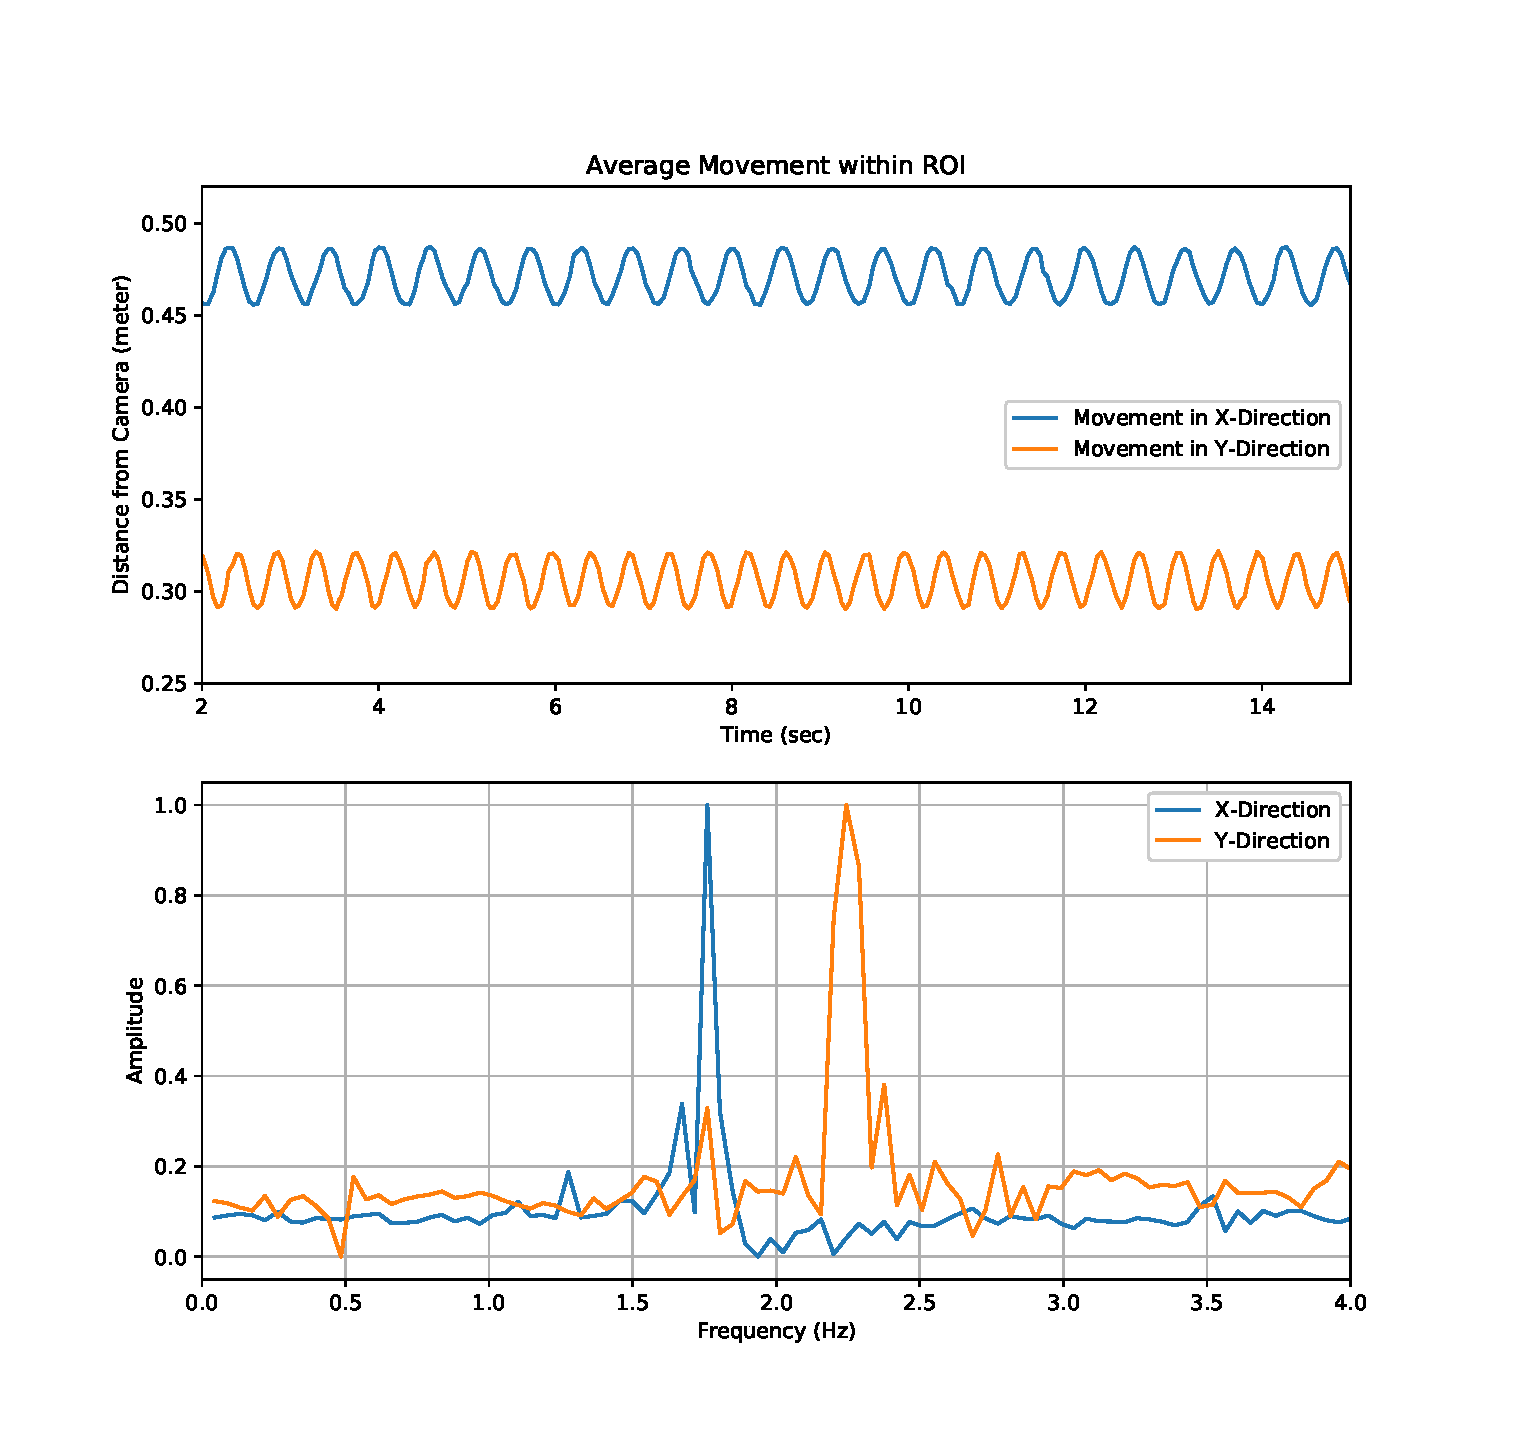
\includegraphics[width=\columnwidth]{Figures/6.eps}
    \caption{Presented Post-Processed Data}
    \label{fig:post}
\end{figure}

To collect the objective metrics of the study, the users filled out a short questionnaire during each test. The questions are listed below:

\begin{enumerate}
    \item Calculated Amplitudes:
    \item Calculated Frequencies:
    \item Which Direction moved fastest?
    \item What is the shape of the motion?
    \item How many seconds did the test last?
    \item How was the frequency found?
\end{enumerate}

For the objective results calculation, questions 1, 2, and 6 were used. Question 6 revealed whether the user guessed the frequency or used the plot of the frequency as they should. Questions 3, 4, and 5 were used as a subjective measure to help assess the understanding of the system. To collect the data, a standard procedure was used for the every user. The procedure of the test is listed below:

\begin{enumerate}
    \item Welcome user and discuss and sign the consent form,
    \item Fill out pre-test questionnaire to assess the user's understanding of vibrations and MATLAB or other programming language on a 5-point Likert scale,
    \item Discuss the four test and present the user with a sample real-time plot to increase understanding of the graphs and outputs of the system,
    \item Randomly assign the data file ordering and the auditory cues ordering,
    \item Perform the three real-time studies,
    \item Perform the post-process study,
    \item Discuss the user's feelings towards the tests as an additional subjective measure,
    \item Discuss the user's results.
\end{enumerate}

\subsection{User-Study Results}

When the users were presented with the real-time data, they had difficulty understanding and interpreting the data; however, when presented with the post-processed data, the users were able to more accurately interpret the results. The results of the correctness is presented in Table \ref{table:resultsus}. If a user was able to correctly estimate the frequency within $\pm0.25$-\textit{Hz}, that user was given a 1 for correctness; however, if the user was not able to estimate the frequency within $\pm0.25$-\textit{Hz} that user was given a 0 for correctness for each test. Moreover, there was not a significant difference between the auditory cues during the real-time studies. The users subjectively reported that the auditory cues, although annoying, did not seem to affect their concentration. There was a difference within the real-time study between the first attempt to interpret the real-time data from the third attempt. Therefore, the user's best score was used from the three real-time tests to calculate the correctness. The mean correctness is plotted in Figure \ref{fig:usresults}. Using an ANOVA test with a within subjects (repeated measure) experiment with eight participants, the results of real-time versus post-processed data interpretation were significant ($F_{1,7}$ = 11.7, $p$ < 0.05). Since users were able to interpret the data more effectively in the post-processed presentation, the Null Hypothesis is rejected. This rejection suggests that the cost of implementing the hardware and software upgrades to provide the real-time data outweighs the benefit to the engineers on the field. Engineers can more effectively and efficiently interpret the data in-office rather than in real-time in the field.

\begin{table}[ht]
\centering
\caption{Results of User-Study}
\label{table:resultsus}
\begin{tabular}{@{}rcc@{}}
\toprule
 & Correctness & Standard Deviation \\ \midrule
Real-Time Data & 25\% & 0.43 \\
Post-Processed & 88\% & 0.33 \\ \bottomrule
\end{tabular}
\end{table}

\begin{figure}[ht]
    \centering
    \includegraphics[width=\linewidth]{Figures/USResults.PNG}
    \caption{Mean Correctness for Real-Time and Post-Processed Data Interpretation}
    \label{fig:usresults}
\end{figure}
 
\section{Summary}

In measuring the dynamics of bridges, the proposed framework and case studies show potential in measuring the dynamic traffic loading and 3-D structural response. First, by using a MOSSE filter, a truck is tracked from a weigh-in-motion sensor on the Interstate Highway in the United States to the test bridge which provides the real-time measurement of loading of the structure. Next, 2-D planar movement and 1-D depth movement measurement techniques are integrated to find the true 3-D displacement of the structure. With both dynamic loading and response known, the performance of the structural system can be better understood. This would allow for better condition assessment and ultimately support decision-making for maintenance and repairs of existing infrastructure by bridge owners and managers. 

Lastly, through a user-study of civil engineers with proficiency in the field of vibrations, it was suggested that users found difficulty interpreting real-time data in the field as opposed to post-processed information.

\section{Future Work}

The proposed framework presented case studies for each module. The entire framework needs to be tested and studied on a bridge with all three modules connected and the performance needs to be studied and further evaluated.

The truck tracking module needs to be tested in an environment with multiple vehicles present. The MOSSE filter is quite robust when tracking one object. But often time, multiple trucks can appear very similar from above. The efficacy of the MOSSE filter, in this case, needs to be tested. Moreover, as the distance from a weigh-in-motion station to the bridge of interest increases, the feasibility of tracking the truck needs to be evaluated considering the limitation of UAV flight distance. The optimal distance needs to be studied to see what type of range is achievable for the proposed system. 

To measure the planar movement of an object, an artificial pattern must be implemented on an object. When applying the technique in the real environment, the implementation of this speckle pattern could become an arduous task negating the benefit of the algorithm. Therefore, to provide a better implementation in the future, other alternatives need to be studied. Concrete and steel are more or less smooth surfaces that do not produce many SIFT key-points. One possibility is to utilize multiple laser projection sensors installed on multiple UAVs to measure depth in different directions to provide the 3-D displacement measurements (i.e. measuring with one artificial laser projection in each x, y, and z-directions). This potential alternative will be investigated. Some limitations with the RealSense Camera need to be considered in the future investigation. Since the RealSense sensor was originally developed for humans interacting with computers, the working distance is rated to 10-\textit{meters}. However, through testing, it was shown that above a working distance of about 3-\textit{meters} the error of the measurement becomes significant. Additionally, the infrared laser and sensors do not work as effectively outside in sunlight; the infrared speckle pattern becomes washed out with the radiation from the sun in outdoor environments. However, working in shady environments outside of direct sunlight, the infrared laser is still captured by the infrared camera. Therefore, the promise of working under a bridge is still viable. Moreover, either a more powerful or different laser type may perform better in outdoor environments. The idea behind the projection of an artificial laser-pattern does show promise to provide a robust technique to measure depth. Therefore, the most appropriate laser type still needs to be studied and examined.

Lastly, although the results of the user-study were significant, more research needs to be done to determine the external validity of the study. For instance, a relatively small number of users were studied. Also, the users studied were not familiar with how the information was displayed nor did they know exactly how the data was collected. Properly priming the users and including more user could provide a different outcome from what was found in this study. 

\section{Acknowledgment}

The work presented in this paper was conducted with support from Colorado State University and the Mountain-Plains Consortium, a University Transportation Center funded by the U.S. Department of Transportation. The contents of this paper reflect the views of the authors, who are responsible for the facts and accuracy of the information presented. (FASTACT Grant No. 69A3551747108). Additionally, the authors would like to acknowledge the UAVs and assistance provided by the Colorado State University's Drone Center. The authors appreciate the experimental testing opportunities provided by the Colorado State University's researcher Dr. Paul Heyliger and his two graduate students Lubna Al Ani and Mohammed Alkharisi. Also, the authors appreciate the sensors and expertise provided by Colorado State  University's researcher Dr. Francisco Ortega.

% REFERENCES FORMAT
\bibliographystyle{SIGCHI-Reference-Format}
\bibliography{ref}

\end{document}
